% Chapter 3

\newglossaryentry{json}{name=JSON, description={JavaScript Object Notation}}
\newglossaryentry{bdb}{name=BDB, description={Python Debugger Framework}}

\chapter{Development} % Write in your own chapter title
\label{chap:development}
\lhead{Chapter 3. \emph{Development}} % Write in your own chapter title to set the page header
\begin{flushright}
\textit{``For me, open source is a moral thing.''} \\ Matt Mullenweg
\end{flushright}

In this chapter, we present the result of our work on the dynamic program analysis. Introduced in the first chapter, the proof-of-concept system is staged here through the explanation of some key code parts and its developed features.

\section{Proposed solution}
While working on a growing project, there is always a point where it becomes difficult to have knowledge about what data is used for. Indeed variables are one of the most important pieces in a source code and in order to give the programmer a better overview of the variables evolution, this work intents to propose a proof-of-concept system which will not only monitor the data evolution, but also give the possibility to compare the gathered data between different runs.

To achieve such a system, the project has been separated in three different components which will constitute the system. First, a data capture process is monitoring all the needed variables and their evolution during the execution of the reviewed program. Then a data model has been created along with a backup procedure which stores the data in this model. Finally, a web-application processes the extracted data and shows them for reviewing the results. Each mentioned part is described in detail in the following sections.

\section{Environment}
In order to achieve the proof-of-concept system, we chose four technologies. First, we used the \textit{Python} programming language to instrument the data. Python is a widely used high level programming language which has seen these last year an increasing enthusiasm around it and is now the most popular introductory teaching language at U.S. top universities according to \cite{Guo2014}. Thanks to the dynamic nature of Python, which includes a dynamic type system, the real-time collection of object is a straightforward process and therefore it made plenty sense to use it for a proof-of-concept application. More over Python offers a handy integrated Debugger Framework and also good compatibility with other programming language since there are a lot of bindings available. For this project, we used the version 3 of Python because of improved encoding handling.

Secondly, the extracted data is stored in a \textit{MongoDB} Database which is a document-oriented database entering in the new category of No-SQL database systems. MongoDB has the advantage to use \gls{json} like documents with schema and consequently this is why we choose it to store the heterogeneous extracted data.

Finally, the user interface is built with the help of \textit{Python}, \textit{HTML/CSS} and \textit{Javascript}. Python is now an interesting language to develop web applications because of his extensive support of libraries and is used here, with the help of the Flask framework, for the server side process. HTML/CSS and Javascript are used for the presentation of the results.

Additionally, the chosen IDE is PyCharm which is a very complete IDE supporting among others Python web frameworks, databases, code inspection. This IDE is essential for the development of our application because it helped us with its good library handling and its integrated version control repository manager. In order to optimize the development management, we choose the GitHub online tool as version control repository. The deployment during the development of the solution was tested on virtual machine server under Ubuntu Server 14.04. 

In order to deploy regularly the newest version of the ongoing work, an automation server named Jenkins was configured. Jenkins is charged to fetch every day the latest prototype on the GitHub repository, create a package of it and install it on the server. If during this process a bug occurs, an e-mail to the interested persons is sent.

In the next section, each module of the proposed system will be exposed in details regarding their functionality and their implementations.

\section{Data Capture Process}
This section presents the crucial developed elements of the data capture process. The data capture process, also called \textit{analyser}, is the core of the system and is based on the Python Debugger Framework (\gls{bdb}). BDB handles basic debugger functions, like setting breakpoints or managing execution. Thanks to the object-oriented features (classes and functions inheritance) of Python, it is a simple task to rewrite the different functionality as needed for this project. The different features are regrouped in a global class which we called \textit{Yoda}.


\subsection{Setting up the trace}
In order to use the analyser, some code has to be added at the beginning of the target file. The code is necessary to import the module and to set the start point of the tracing phase. 
\begin{python}
import yoda.analyser
yoda.analyser.db.set_trace()
\end{python}

The \pythoninline{set_trace()} function is inherited from the BDB and is needed to start debugging with a Bdb instance from a caller’s frame.
It is also necessary to stop the trace at the end of the target code with the \pythoninline{yoda.analyser.db.set_quit()
} function which set the quitting attribute to \texttt{True}. This raises BdbQuit exception in the next call to one of the \pythoninline{dispatch_*()} methods with the goal to prevent further tracing. Indeed, even if the complete file is analysed, this needs absolutely to be set to avoid unexpected further analysis. 

The detailed information about the operating of the Python Debugger Framework, is provided in the official documentation \citep{Foundation2017}.

\subsection{Initialization}

Once the analyzer module is called, the trace is automatically started. The first background step operated by the system is to setup the \pythoninline{Yoda} class along with some global variables needed during the tracing process. The first variable \pythoninline{json\_results} (line 2) will be explained further but is basically where the extracted data will be stored. Then, the \pythoninline{instrumented\_types} list (line 3) limits the amount of instrumented objects to the given set, it is possible to add further objects if needed. The next 6 variables (line 4-9) are needed for gathering and computing the line numbers, frames and files name. Finally, the \pythoninline{next_backup} variable (line 10) defines a limit of how many lines can be analyzed before flushing the information in the database.

\begin{python}
class Yoda(bdb.Bdb):
    json_results = None
    instrumented_types = (int, float, str, list, dict)
    prev_lineno = defaultdict(int)
    prev_lineno['<module>'] = 0 
    cur_framename = '<module>'
    file_name = None
    file_id = None 
    total_linenb = 0
    next_backup = 1000
\end{python}

As the needed variables are now set up, the script continues with the initialization of the \pythoninline{Yoda} class. Within the class, the connection of the database is created when the system is configured for production mode (line 4). 

\begin{python}
def __init__(self):
    bdb.Bdb.__init__(self)
    if settings.DEBUG is False:
        mongoengine.connect(settings.MONGODB)
\end{python}

\subsection{Event Catching}

BDB can react to various events during the code execution which are handled by 4 functions : \texttt{user\_call, user\_line, user\_return, user\_exception}. Each function has been overridden in order to redirect the event to a special handling function called \texttt{interaction}. 
\smallskip
\begin{python}
def user_call(self, frame, args):
    self.interaction(frame, 'call', None)
def user_line(self, frame):
    self.interaction(frame, 'line', None)
def user_return(self, frame, value):
    self.interaction(frame, 'return', None)
def user_exception(self, frame, exception):
    self.interaction(frame, 'exception', exception)
\end{python}

Once the \texttt{interaction} function has been called, the first thing the system does is to check whenever the \texttt{file\_name} variable is blank or not. If \texttt{file\_name} is \texttt{None}, then a new one is retrieved and applied from the source code file, otherwise the script will continue with the handling of the events.
\begin{python}
if self.file_name is None:
    self.file_name = inspect.getfile(frame)
\end{python}

\subsection{Event Handling}
The first handled event type is the \texttt{call} type. This kind of event is normally happening when the frame of the code is changing and thus there is not much to do. Indeed, it just need to capture the frame name (line 2) and catch the line number (line 3). Nothing else special is handled there.
\begin{python}
if event == 'call':
    self.cur_framename = str(frame.f_code.co_name)
    self.prev_lineno[self.cur_framename] = frame.f_lineno
    self.set_step() # continue
\end{python}

The succeeding event type is the the \texttt{line} type which occurs at each line-break. This event is vital for the data collection and therefore its operating has to be explained separately. First, the interaction function, as before, checks the type of the event and then proceeds to extract the line number which is a key information for the user interface. Then for each line, the interpreted objects have to be caught. This is handled by a external function called \texttt{\_filter\_locals} and called with the frame locals as an argument.
\begin{python}
locals = self._filter_locals(frame.f_locals)
\end{python}

The function itself first creates an empty dictionary which will store the name and the value of each local variable (line 2). The locals starting with a double underscore are ignored and only the specified objects are fetched (line 4 to 6). The function returns the \texttt{new\_locals} dictionary to the main \texttt{interaction} function (line 9).

\begin{python}
def _filter_locals(self, local_vars):
    new_locals = {}
    for name, value in list(local_vars.items()):
        if name.startswith('__'):
            continue
        if not isinstance(value, self.instrumented_types):
            continue
        new_locals[name] = [copy.deepcopy(value)]
    return new_locals

\end{python}

Then, the locals are stored in a JSON defaultdict object along with the file name, the frame and the line number. At the end, the JSON dictionary is periodically stored in the database in order to flush the data from the memory and enhance the runtime performance. The population of the database is detailed in the next section.

\begin{python}
if self.total_linenb > self.next_backup:
    self._populate_db()
    self.next_backup += self.next_backup
\end{python}

The handling of the \texttt{line} event is now finished and the interaction function continues with the two last types. The \texttt{return} event only occurs at the beginning of a file for which we just set the main frame name (line 2) and the \texttt{exception} event happens when there is an error in the code which is printed out in the console (line 6).
\begin{python}
if event == 'return':
    self.cur_framename = '<module>'
    self.set_step()  # continue
if event == 'exception':
    name = frame.f_code.co_name or "<unknown>"
    print("exception in", name, exception)
    self.set_continue()  # continue
\end{python}

\subsection{Trace Ending}

Finally, the data capture model is ended by the \pythoninline{set_quit()} BDB function which was remodelled for writing the last traced lines (line 7-11).
\begin{python}
def set_quit(self):
    self.stopframe = self.botframe
    self.returnframe = None
    self.quitting = True
    sys.settrace(None)

    if self.json_results:
        if settings.DEBUG:
            print(self.json_results)
        else:
            self._populate_db()
\end{python}



\section{Data model}
The data model is an in-between layer used for the Data capture model and the user interface. Both modules parts will be explained in this section along with the presentation of the data model itself.

\subsection{Definition}
The data model itself evolved a lot during the development and lead to the finale state which will be presented here. This can be observed in the chosen nomenclature, which sometimes does not exactly correspond to the reality. The best example is the use of the substantive "file" in the code which actually describes more an analysis instance or a run than the file itself. Thanks to the MongoDB database engine, it is easy to modify the document structure without any database manipulation in contrary to the data structure of relational database systems. This was a great asset which allowed significant time savings in the development of the data model since it changed a many times.

To understand the data model it is a good reminder to enumerate what the data capture model is actually capturing. First the model is searching for objects, i.e. integers, strings and floats variables including for each type their values. These objects are linked with line numbers, which are them-self linked with frames. Finally, each frame is owned by a file (or more specifically a run as it was pointed out previously).

Keeping that in mind the different data structures can be considered as documents and defined the following way in Python. This notation is used further for reading from the database. First, the \textit{line} which has a number and some data (objects):
\begin{python}
class Line(EmbeddedDocument):
    lineno = IntField()
    data = DictField()
\end{python}

Secondly, the \textit{frame} which has a name and contains one or many lines :

\begin{python}
class Frame(EmbeddedDocument):
    name = StringField()
    lines = ListField(EmbeddedDocumentField(Line))
\end{python}

Finally, the \textit{file} which has a name, a time-stamp, the content itself (source code) and additionally a revision number gathered from the git repository when available and also the user name of the person who started the analysis. The file contains logically the different frames and is defined in the following way :
\begin{python}
class File(Document):
    user = StringField()
    revision = StringField()
    filename = StringField()
    timestamp = DateTimeField()
    content = StringField()
    frames = ListField(EmbeddedDocumentField(Frame))
\end{python}

\subsection{Writing to the database}
This part of the database handling is directly implemented in the data capture model along with the capture functionality. The process can be called in two different states of the analysis phase : 
\begin{itemize}
  \item The program reached the limit of lines and needs to flush the gathered data into the database. This occurs inside the \pythoninline{interaction()} function which has already been described in the previous section
  \item The system reached the end of the analysed file and the function \pythoninline{set\_quit()} has been called.
\end{itemize}
Both states induce the call of the \pythoninline{\_populate\_db()} which is constituted of an \pythoninline{if...else} condition. This condition checks whenever it is the first time the system tries to backup the data or not and calls respectively the \pythoninline{\_create\_new\_file()} or the \pythoninline{\_update\_file()} functions (line 3 and 6).
\begin{python}
def _populate_db(self):
    if self.file_id is None:
        self._create_new_file()
        self._clear_cache()
    else:
        self._update_file()
        self._clear_cache()
\end{python}

If the system needs to create a new document in the database, as already stated it will call the \pythoninline{\_create\_new\_file()} which is explained here in a simplified and step-by-step version. The complete version of the function includes also a compatibility layer for Python 2 but we removed it here for readability reasons. The first step of the creation of a new entry is to fetch each row of the JSON type dictionary (line 2), where the system stored the data  until now, and split the data in two separate variables (\pythoninline{module\_file} and \pythoninline{frames}).
\begin{python}
def _create_new_file(self):
  for module_file, frames in self.json_results.items():
\end{python}
 
Then, in order to display also the source code in the user interface, we retrieve the content of the file (line 1-3). Finally, we gather the \pythoninline{user} and the \pythoninline{revision} variables with the git command line tool and create the file object in the database (line 4).
\begin{python}
file = open(module_file, 'r')
file_content = file.read()
file.close()

item = File(user=self._get_git_username(), revision=self._get_git_revision_short_hash(), filename=module_file, timestamp=datetime.now(), content=file_content)
\end{python}

The next step is to create the \pythoninline{frame} document (line 2) along side with each \pythoninline{line} document belonging to this frame (line 4). Finally, we link the frame to the file (line 6) and save the file into the database (line 7). Additionally the variable \pythoninline{file\_id}, which was previously defined, is set.
\begin{python}
for name, lines in sorted(frames.items()):
    frame = Frame(name=name)
    for lineno, data in sorted(lines.items()):
        line = Line(lineno = lineno, data = data)
        frame.lines.append(line)
    item.frames.append(frame)
    item.save()
self.file_id = item.id
\end{python}

Now that we created a first backup in the database for our run, the system will eventually have to update the database with the following analysed lines and therefore it will call again the \pythoninline{_populate_db()} function. This time, because the system set the \textit{file\_id} variable just before, the \pythoninline{\_update\_file()} function is called. We implemented this function in a similar way as the \pythoninline{\_create\_new\_file()} one. First, as in the earlier function the JSON dictionary is looped in order to gather the needed data.
\begin{python}
def _update_file(self):
  for module_file, frames in self.json_results.items():
\end{python}

Then for each frame, the system first checks if it is a new frame or not (line 2) and hence creates it in the database (line 3-4). Finally, we create the new analysed lines and save them in the database (line 5-7).
\begin{python}
for name, lines in sorted(frames.items()):
    if not File.objects(id=self.file_id, frames__name=name):
        frame = Frame(name=name)
        File.objects(id=self.file_id).update(push__frames=frame)
    for lineno, data in sorted(lines.items()):
        line = Line(lineno = lineno, data = data)
        File.objects(id=self.file_id, frames__name=name).update(push__frames__S__lines=line)
\end{python}

\subsection{Reading from the database}

Reading from the database exclusively arises in the user interface module. In standardise the procedure, we chose to use the \textit{MongoEngine} library. The MongoEngine is a Document-Object Mapper for working with MongoDB in Python. Thanks to the use of this library, it is possible to gather the data of a run in the database only with one line of code.
\begin{python}
file_object = File.objects(id=file_id)
\end{python} 

This line of code gathers the complete data of a run, but thanks to the API of MongoEngine it is also possible to retrieve specifically the needed data. If these special options are in the interest of the reader, we suggest to refer directly to the MongoEngine documentation.

\section{User interface}
The user interface is a web application which helps the programmer to review the result of the data capture model. In this section,  we decided to focus on the features rather than on the code for different reasons. First, we do not consider the user interface code here as the core knowledge of the developed system. Then the complete web application represents almost 1000 lines of code and would stretch considerably out this report with few added value. Finally a non negligible part of the code fulfils a visual and presentation purpose rather than actual features.

\subsection{Technologies}
The web application is based on the Python web framework \textit{Flask} which is intended to be as lightweight as possible. The flask micro-framework comes with some handy features such as built-in development server and debugger, integrated unit testing support, RESTful request dispatching, or \textit{Jinja2} templating. Flask is normally designed to connect with standard SQL databases but with the help of the \textit{flask-mongoengine} extension the process is pretty straightforward.

The shaping of the web-application is indeed done with the help of \textit{HTML/CSS} and \textit{Javascript}. For purposes of standardization, the \textit{Bootstrap} framework came in help which includes also the convenient \textit{JQuery} javascript framework. Bootstrap is a popular HTML, CSS, and JS open-source framework for developing front-end projects on the web. As for Jquery it is a fast, small, and feature-rich JavaScript library which makes things like HTML document traversal and manipulation, event handling, animation, and Ajax much simpler with an easy-to-use API that works across a multitude of browsers.

Some other libraries came also during the development to format the data out of the database. With this aim in mind, we first used the DataTables library which makes formatting data in table a child's play. Additionally we are using the \textit{Highcharts} Javascript library to generate every graphs and \textit{pygments} to highlighting the Python syntax.

\subsection{The cockpit}
The user interface is composed of three main pages. The first one, represented by the \autoref{fig:home}, is the index page which shows an overview of the different runs stored in the database. This page also acts as a cockpit which allows the user to view runs in detail, select runs for comparison and to delete unwanted runs from the database. The runs are searchable and can be sorted by dates, file name, Git revision or user name. It is also possible for the user to configure how many runs should be shown per page.
\begin{figure}[h!]
  \centering
    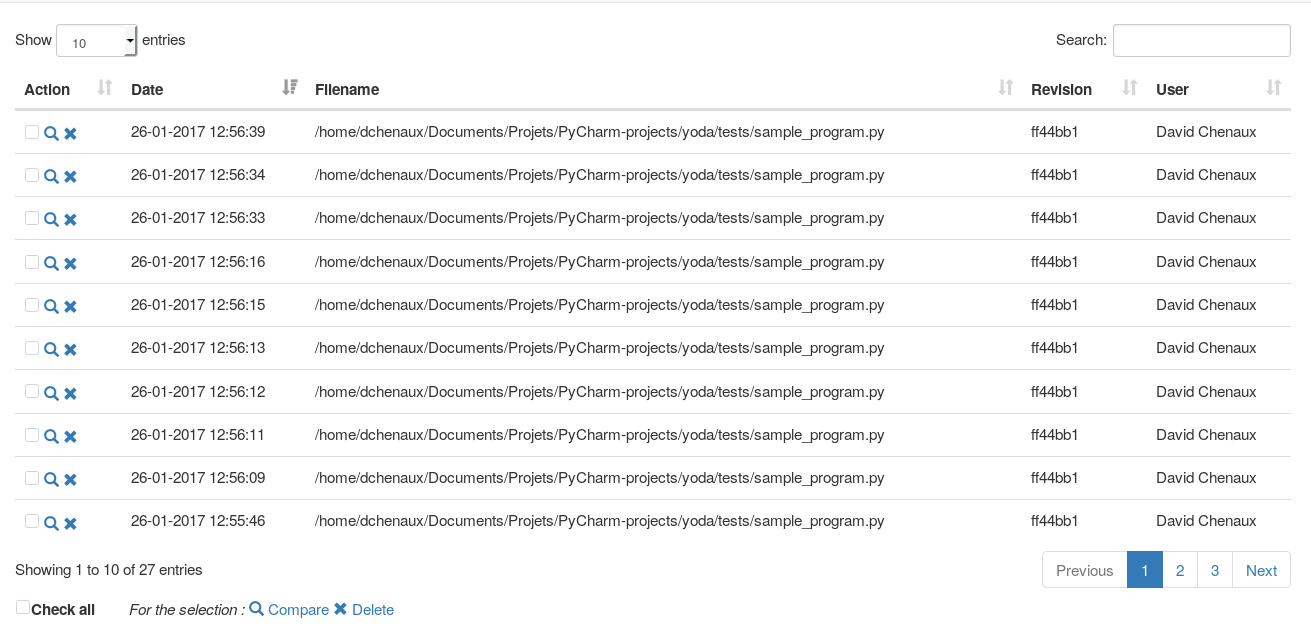
\includegraphics[width=\textwidth]{figures/yoda-home.png}
    \caption{The cockpit}
    \label{fig:home}
\end{figure}

\subsection{The file reviewer}
Once the user selected a run in the cockpit, he will be directly redirected to a the corresponding results page as illustrated by the \autoref{fig:viewafile}. 
\begin{figure}[h!]
  \centering
    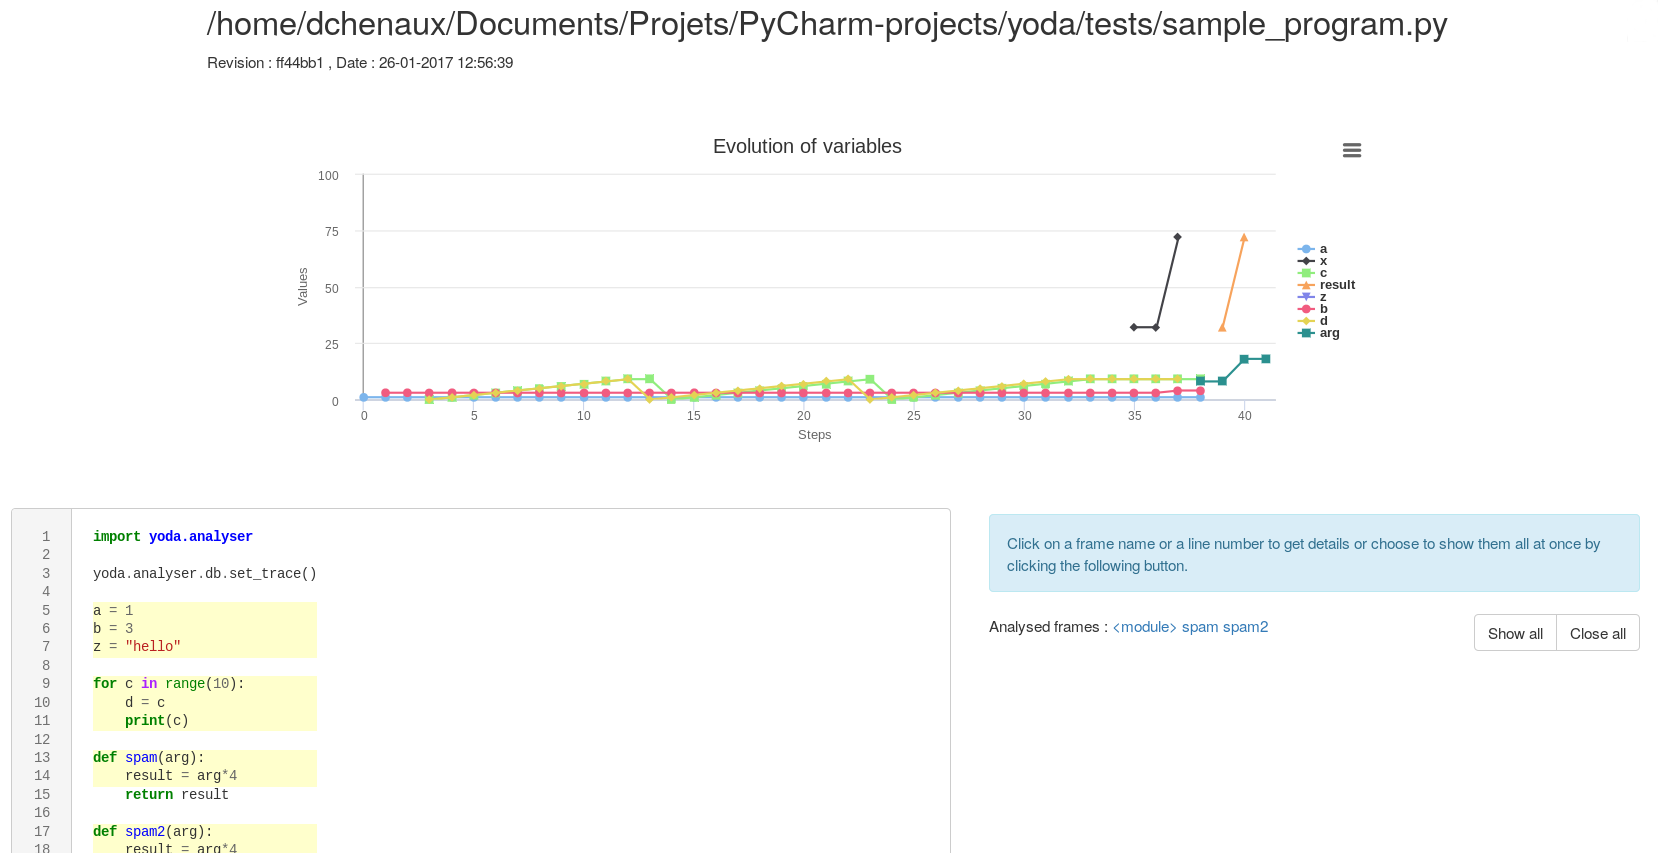
\includegraphics[width=\textwidth]{figures/yoda-file.png}
    \caption{Reviewing a file}
    \label{fig:viewafile}
\end{figure}

This page is separated in 4 main sections. First, at the head of the page there is some basic information about the run such as the file name, the date of the run or the git revision. Directly underneath, when possible, a plot graph is computed and shows by default all the available objects. The user can choose to hide some variable and the scope of the graph is automatically adapted to the remaining values. Additionally, the chart can also be printed and exported in several different formats.

Next, in two vertical columns, the user will find in the left part the complete source code of the analyzed file. The pieces of code which were genuinely analyzed are highlighted in a light yellow color and moreover every line has been numbered and syntactically colored. The line numbers are clickable and open a panel in the right column with some further information about the analyzed objects. Each panel contains a header with the frame name and the line number, and a body with the objects names, their values and a small inline graph representing the evolution of the value. The \autoref{fig:filefocus} shows in detail these described features. Additionally on the top of the right column some buttons allow to show all the panels, close them or selectively open all panels linked to a frame.

\begin{figure}[h!]
  \centering
    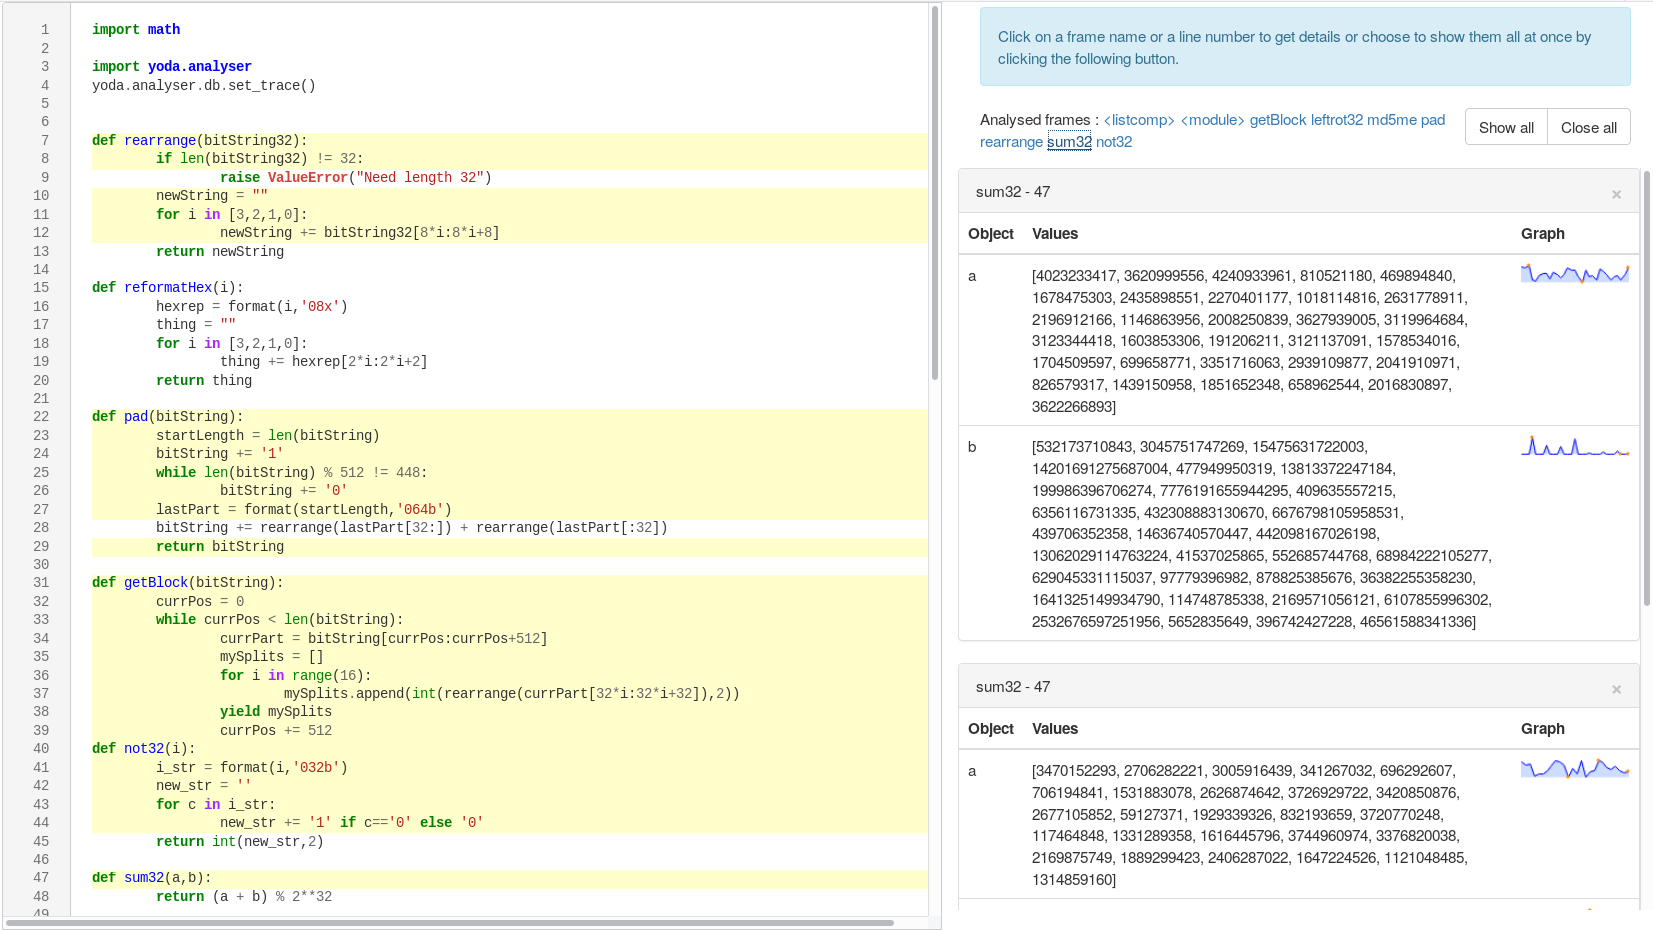
\includegraphics[width=\textwidth]{figures/yoda-file-focus.png}
    \caption{Sources code and detail panels}
    \label{fig:filefocus}
\end{figure}

\subsection{File comparison}
If needed the user has also the possibility to select several files in the cockpit in order to compare them. This is done by checking the needed runs and clicking the "compare" link at the bottom of the page. Doing so will redirect the user to the start page of the comparison. From this page, each file can be inspected and the user is given the choice of which object he wants to select for the comparison as shown on the \autoref{fig:comparisonstart}.
\begin{figure}[h!]
  \centering
    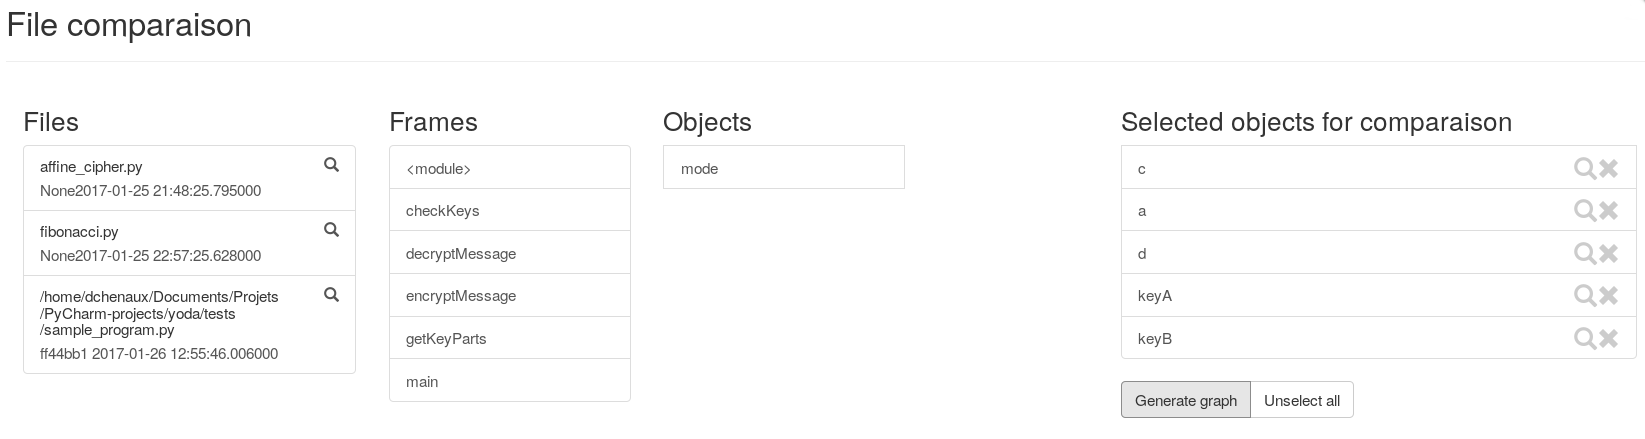
\includegraphics[width=\textwidth]{figures/yoda-comparison.png}
    \caption{Runs comparison}
    \label{fig:comparisonstart}
\end{figure}

For each selected object, the user has the possibility to see the source file or eventually to deselect it. When he is happy with his selection, graphs can be generated with the triggering of the "Generate graphs" button. For each run a graph will be created and displayed in a way which facilitates comparison as shown on \autoref{fig:generatedgraphs}.
\begin{figure}[h!]
  \centering
    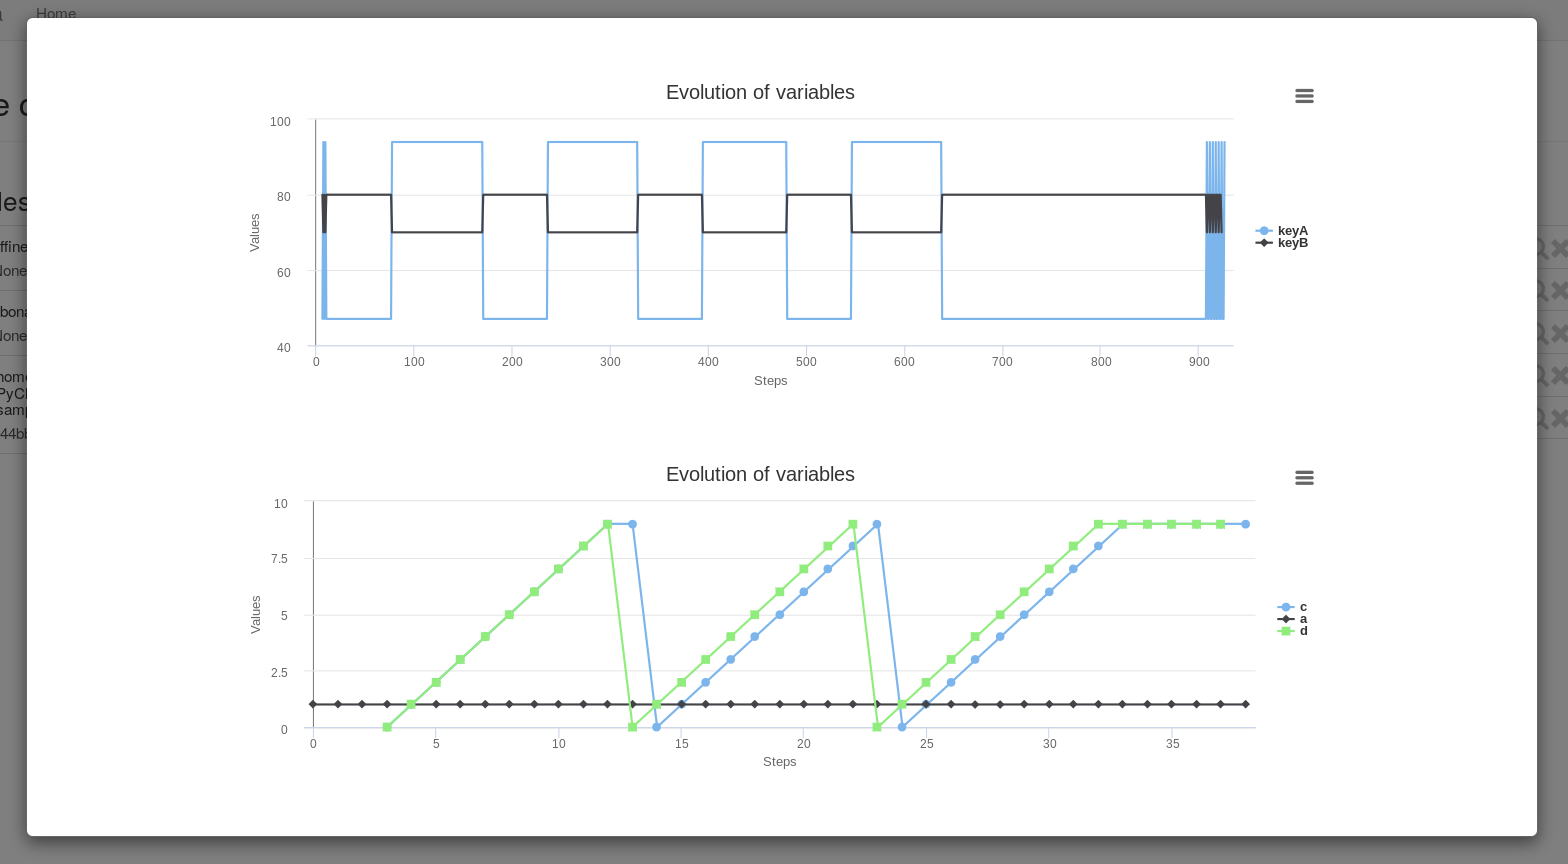
\includegraphics[width=\textwidth]{figures/yoda-graphs.png}
    \caption{Generated graphs for comparison}
    \label{fig:generatedgraphs}
\end{figure}

\section{Concluding remarks}
In this chapter, we gave a brief but complete insight of the implementation of our solution. It was quite a challenge to summary 6 months of development, over 2000 lines of code in a short and comprehensive chapter. We hope we were able to give the reader a good insight of operating method of our developed system. In the next chapter, we are giving a complete guide to install and start the system.
